\PassOptionsToPackage{table}{xcolor}
\documentclass[12pt,letterpaper,twocolumn,openany,nodeprecatedcode,bg=none]{dndbook}
\usepackage[english]{babel}
\usepackage[utf8]{inputenc}
\usepackage{longtable,booktabs,array}
\usepackage{calc}
\usepackage{etoolbox}
\usepackage{caption}
\usepackage{float}
\usepackage{graphicx}
\usepackage{needspace}
\usepackage{tikz}

% Reset zebra striping at the start of every table
\AtBeginEnvironment{longtable}{\rowcolors{1}{white}{gray!10}\small}
\AtBeginEnvironment{table}{\rowcolors{1}{white}{gray!10}}

\providecommand{\pandocbounded}[1]{#1}
\providecommand{\tightlist}{%
  \setlength{\itemsep}{0pt}\setlength{\parskip}{0pt}}

\captionsetup{labelformat=empty}
\setcounter{secnumdepth}{0}
\setlength{\parindent}{0pt}
\setlength{\parskip}{0.5\baselineskip}
\setlength{\headheight}{15pt}

% Prevent orphaned subsections
\let\oldsubsection\subsection
\renewcommand{\subsection}[1]{%
  \needspace{5\baselineskip}%
  \oldsubsection{#1}%
}

\begin{document}
\onecolumn

      \title{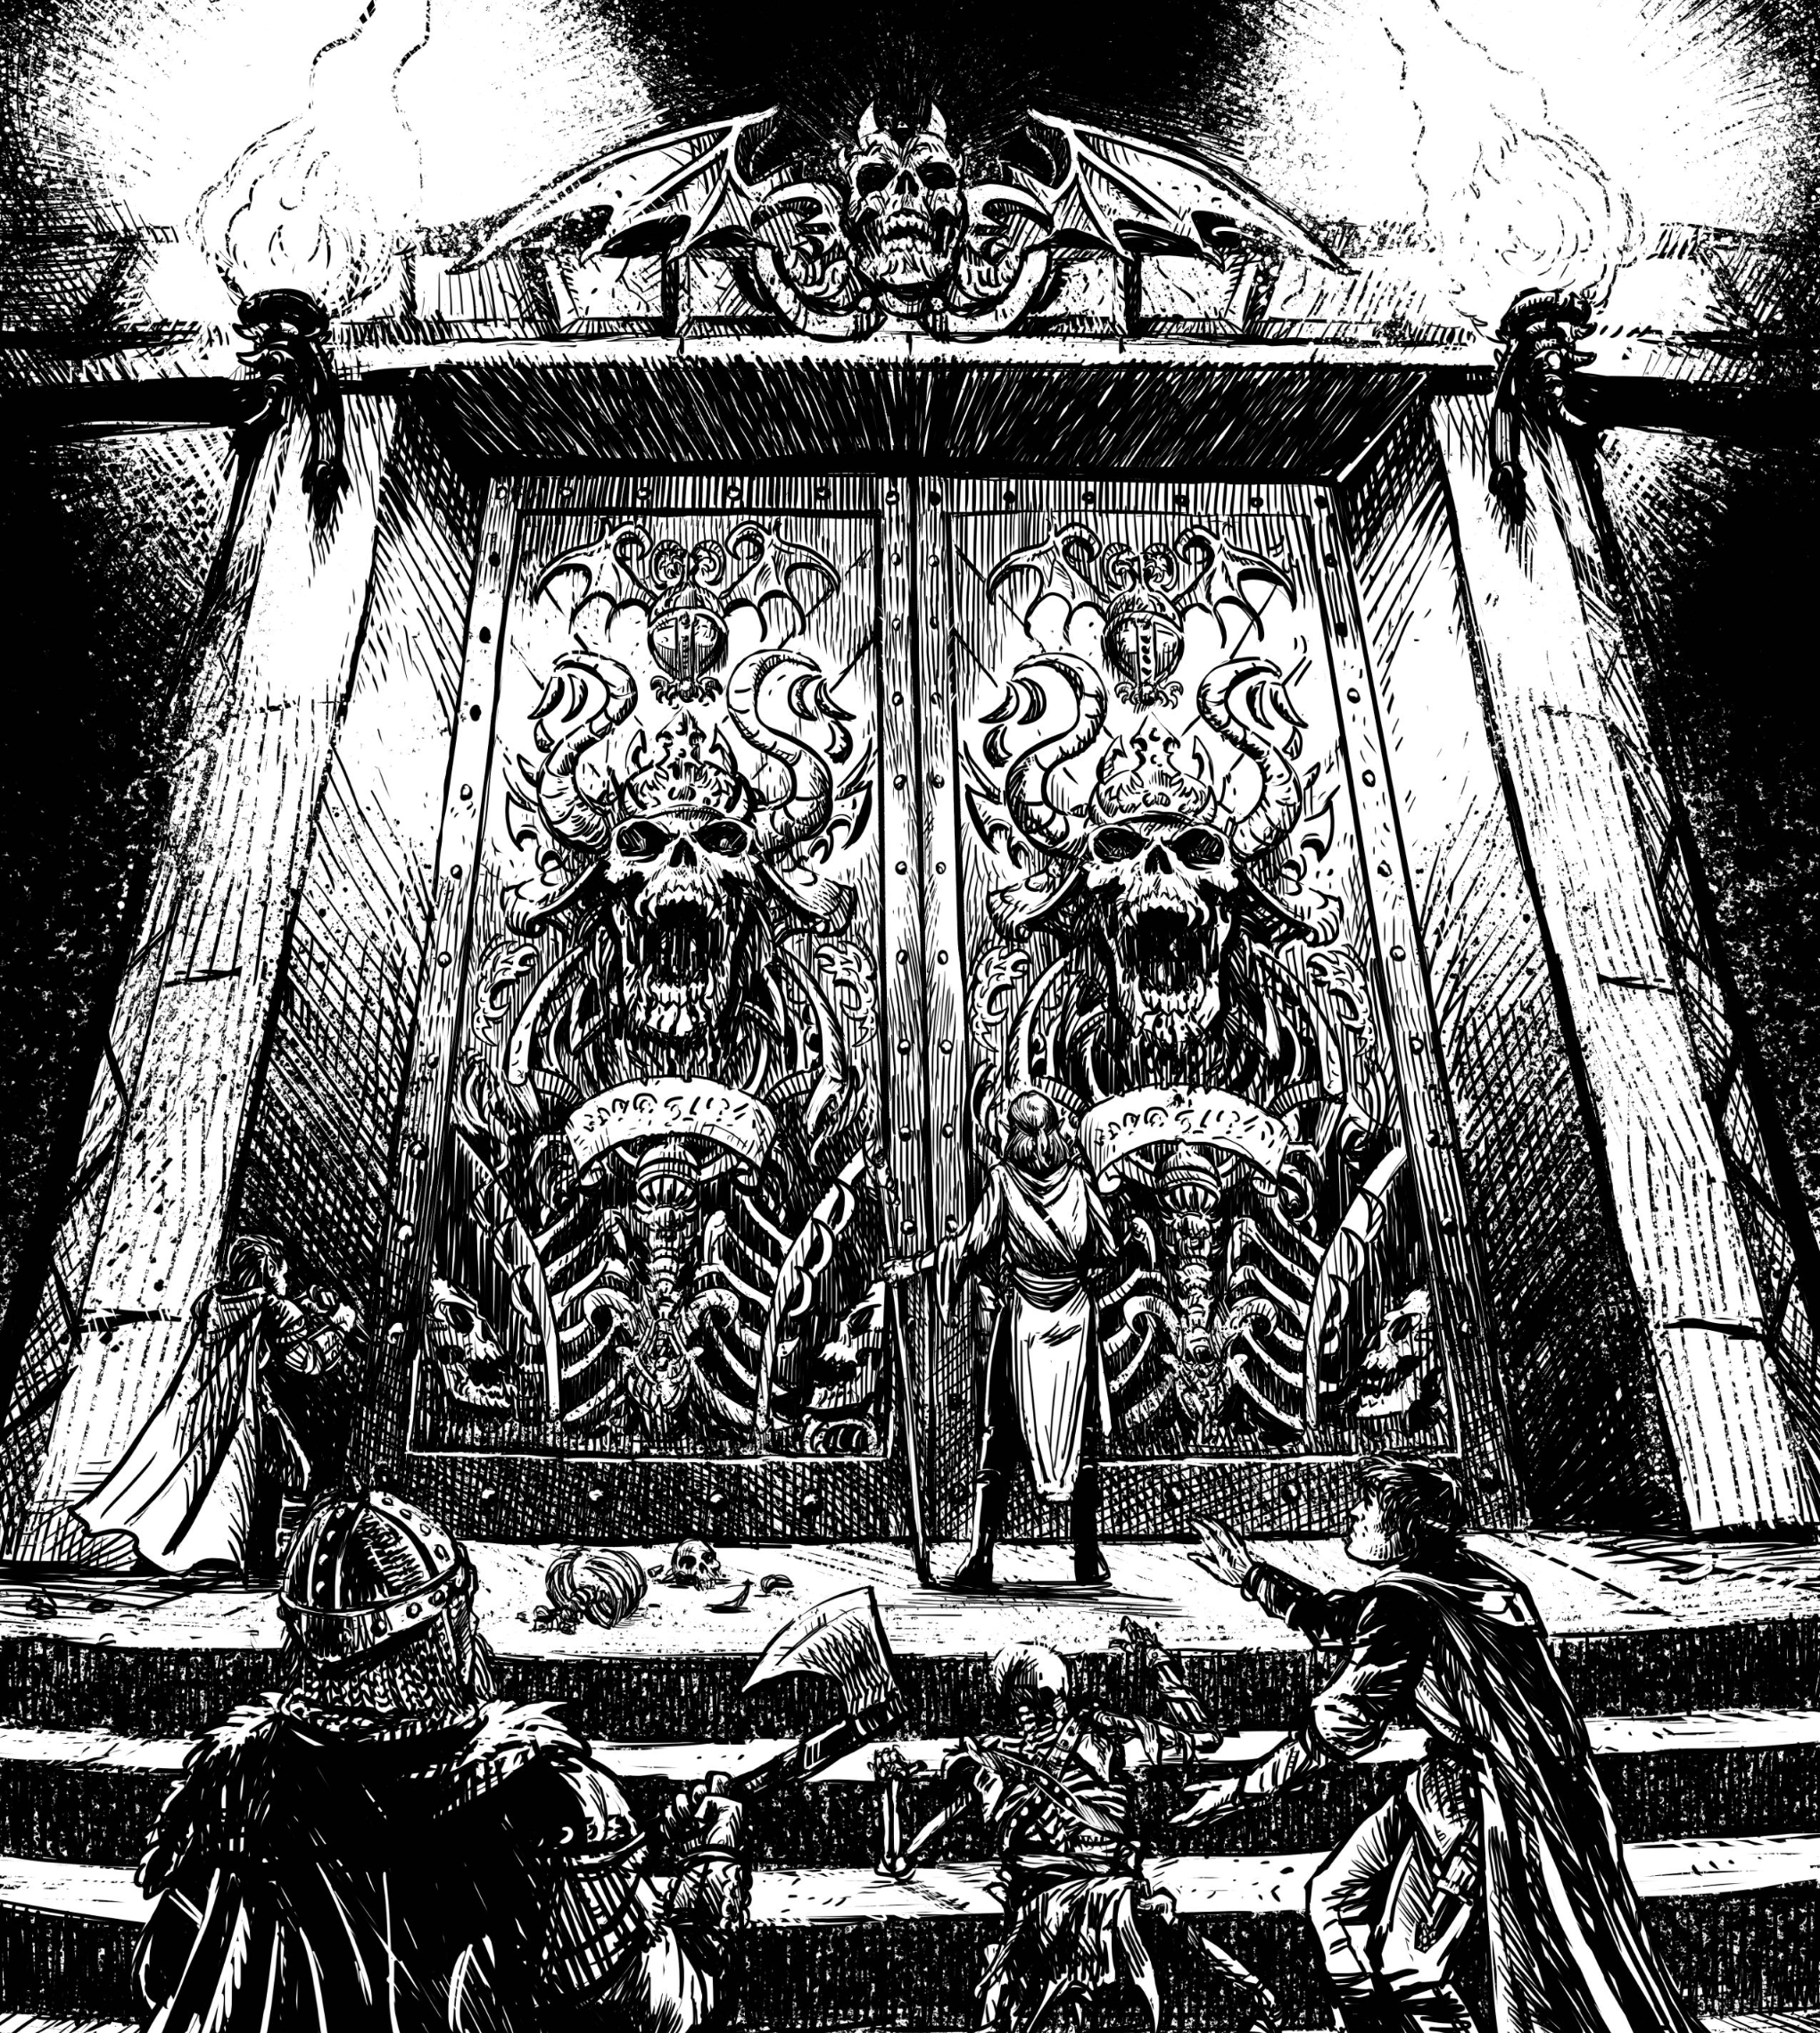
\includegraphics[width=0.9\textwidth,height=0.55\textheight,keepaspectratio]{dungeonDoor.png}\\[1.5cm]Character
Creation}
  \author{Player Handbook}
\date{}
\maketitle

\clearpage
\thispagestyle{empty}
\null\vfill
\begin{center}{\Large\itshape Your trusty player handbook for fantasy
gaming.}\end{center}
\vfill

\clearpage
\thispagestyle{empty}
\begin{center}
\vspace*{\fill}
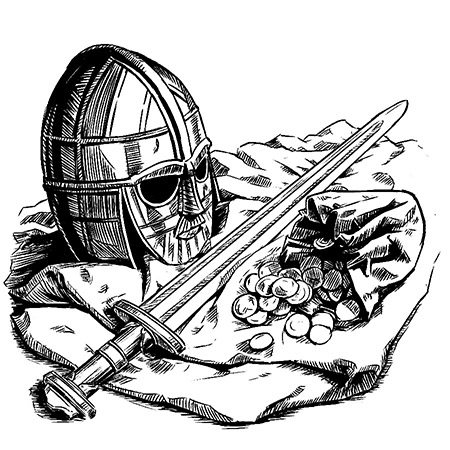
\includegraphics[width=\textwidth,height=0.85\textheight,keepaspectratio]{helmSwordGold.jpg}\par
\vspace{0.4cm}
{\itshape Ancestries, equipment, star signs, and more!}\par
\vspace*{\fill}
\end{center}

\clearpage
\twocolumn

\section{Character Creation}\label{character-creation}

Use the following steps to create a character.

\subsection{The Six Abilities}\label{the-six-abilities}

\textbf{Strength} measures physical might and power.

\textbf{Dexterity} measures agility, coordination, reflexes, and
balance.

\textbf{Constitution} gauges health and durability.

\textbf{Intelligence} reflects logical reasoning, memory, and knowledge.

\textbf{Wisdom} measures intuition, insight, and willpower.

\textbf{Charisma} reflects personal magnetism and charm.

\subsection{Determine Abilities}\label{determine-abilities}

Roll six d6s and allocate each die to a different ability, choosing how
to allocate them or doing it at random. Use the table below to determine
their abilities. Then allocate 2 points to your abilities, with each
point granting +1. You can allocate both points to the same ability for
a +2 bonus.

\needspace{9\baselineskip}

{\def\LTcaptype{none} % do not increment counter
\begin{table}[!htbp]
\centering
\begin{tabular}{@{}
  >{\raggedright\arraybackslash}p{(\linewidth - 2\tabcolsep) * \real{0.1875}}
  >{\raggedright\arraybackslash}p{(\linewidth - 2\tabcolsep) * \real{0.8125}}@{}}
\toprule\noalign{}
\begin{minipage}[b]{\linewidth}\raggedright
d6
\end{minipage} & \begin{minipage}[b]{\linewidth}\raggedright
Ability Score
\end{minipage} \\
\midrule\noalign{}
1 & -1 \\
2 & +0 \\
3-4 & +1 \\
5-6 & +2 \\
\bottomrule\noalign{}
\end{tabular}
\end{table}
}

If you did not roll at least one 5 on your six d6 rolls, you may
re-roll.

\subsection{Class}\label{class}

Choose one of the available Classes that fits with your character's
abilities.

\subsection{Ancestry}\label{ancestry}

You can pick one of the ancestries listed below. Your size is Medium and
your creature type is humanoid. You know the Common language and one
language or dialect that makes sense in the world as determined by both
you and the DM.

\subsubsection{Catfolk}\label{catfolk}

\textbf{Nocturnal.} You have Darkvision with a range of 60 feet.

\textbf{Claws.} You can use your claws as natural weapons for your
Unarmed Strikes. They have the finesse property and you count as being
proficient with them when attacking. They deal 1d6 slashing damage on a
hit.

\subsubsection{Elf}\label{elf}

\textbf{Elven Background.} Pick one of the following options.

\begin{itemize}
\tightlist
\item
  \textbf{Fleet of Foot.} You gain proficiency with Dexterity saves and
  one related skill. If your class grants you proficiency with such
  saves or skills, you instead gain expertise with them.
\item
  \textbf{Resilient Body.} You gain proficiency with Constitution saves
  and one related skill. If your class grants you proficiency with such
  saves, you instead gain expertise with them.
\item
  \textbf{Wizened Mind.} You gain proficiency with Wisdom saves and one
  related skill. If your class grants you proficiency with such saves,
  you instead gain expertise with them.
\end{itemize}

\textbf{Arcane Soul.} You know one cantrip of your choice from any spell
list. Choose any stat as your casting stat for it.

\subsubsection{Human}\label{human}

\textbf{Jack of all Trades.} Increase your proficiency bonus by +1.

\subsubsection{Lizardfolk}\label{lizardfolk}

\textbf{Scales.} Your scales give you +1 AC.

\textbf{Amphibious.} You can breathe both water and air.

\textbf{Reptilian.} You gain resistance to poison damage.

\subsubsection{Orc}\label{orc}

\textbf{Orcish Determination.} On your turn, you can enter a focused,
determined state. For the next 10 minutes you gain advantage on all
attacks, checks, and saving throws. You also gain a bonus to damage
rolls equal to half your level (minimum +1). Once you use this feature,
you cannot use it again until you finish a long rest.

\textbf{Indomitable.} On your turn, you can tap into a well of energy
and toughness. You regain 1d8 + your Constitution modifier hit points.
This amount increases by 1d8 when you reach level 5 (2d8) and 9 (3d8).
Once you use this feature, you cannot use it again until you finish a
long rest.

\subsection{Background}\label{background}

You have decided to embark on a life of adventure. Why grind away at a
mundane career when you can risk life and limb in search of treasures
hidden in monster infested holes in the ground? You background
determines your skills and languages.

\subsubsection{Skills}\label{skills}

You select one of the skill packages listed below.

\begin{itemize}
\tightlist
\item
  \textbf{Merchant}: Deception, Insight, Performance, Persuasion
\item
  \textbf{Scholar}: Arcana, History, Medicine, Religion
\item
  \textbf{Soldier}: Athletics, Intimidation, Medicine, Perception
\item
  \textbf{Thief}: Athletics, Investigation, Sleight of Hand, Stealth
\item
  \textbf{Wanderer}: Animal Handling, Nature, Perception, Survival
\end{itemize}

With your DM's permission, you can create your own skill package by
picking four skills.

Expertise and Ancestry. If your background gives you a skill granted by
your ancestry, you gain expertise with that skill.

\subsubsection{Languages}\label{languages}

You know Common. The DM may provide you a list of languages in their
world that scholar's might reasonably study. If they do, you may choose
a number of those languages to learn equal to to your Intelligence
modifier (minimum 0).

\paragraph{Known Languages}\label{known-languages}

Common, High Elvish, Dark Elvish, Wood Elvish, Orcish, Saxhleel, Taagra,
and Daedric.

\subsection{Star Sign}\label{star-sign}

Choose your Star Sign, what constellation were you born under?

\subsection{Equipment}\label{equipment}

You start with a belt pouch, and a pack of choice. There is one pack for
each of the 5 standard backgrounds; bard's pack, scholar's pack,
soldier's pack, thieves' pack, and a wanderer's pack. Each contains
basic adventurer equipment like torches and rations along with a few
special items tailored to their specific context. Your class grants you
starting weapons and armor.

\needspace{11\baselineskip}

{\def\LTcaptype{none} % do not increment counter
\begin{table}[!htbp]
\centering
\begin{tabular}{@{}
  >{\raggedright\arraybackslash}p{(\linewidth - 2\tabcolsep) * \real{0.1977}}
  >{\raggedright\arraybackslash}p{(\linewidth - 2\tabcolsep) * \real{0.8023}}@{}}
\toprule\noalign{}
\begin{minipage}[b]{\linewidth}\raggedright
Pack
\end{minipage} & \begin{minipage}[b]{\linewidth}\raggedright
Bonus Items
\end{minipage} \\
\midrule\noalign{}
Merchant's Pack & Scale, Lockbox, Fine Clothes, Mirror \\
Scholar's Pack & Book, Ink pen, 10 pieces of parchment and envelopes,
Signet ring, Wax \\
Soldier's Pack & Crowbar, Rope (50'), 8 oil flasks \\
Thieves' Pack & Crowbar, Thieves' Tools, Bag of ball bearings, 10
caltrops \\
Wanderer's Pack & Tent, Hunting trap, Rope (50') \\
\bottomrule\noalign{}
\end{tabular}
\end{table}
}

\section{Equipment}\label{equipment-1}

This section provides the rules for equipment that characters can buy.

\subsection{Weight}\label{weight}

Generally speaking, your total carry weight is not expected to be
tracked exactly at the pound granularity. Instead, the number of pounds
a character can carry is intended to serve as a reference point for how
much stuff they can have on them given their size, strength, and
equipment. The DM ultimately determines what can and can't be carried
based on the situation.

\subsection{Coins}\label{coins}

The table below summarizes the values of the standard coins. 100 coins
weighs roughly 2 pounds and fit neatly into a small purse or bag.

\needspace{9\baselineskip}

{\def\LTcaptype{none} % do not increment counter
\begin{table}[!htbp]
\centering
\begin{tabular}{@{}
  >{\raggedright\arraybackslash}p{(\linewidth - 2\tabcolsep) * \real{0.6552}}
  >{\raggedright\arraybackslash}p{(\linewidth - 2\tabcolsep) * \real{0.3448}}@{}}
\toprule\noalign{}
\begin{minipage}[b]{\linewidth}\raggedright
Coin
\end{minipage} & \begin{minipage}[b]{\linewidth}\raggedright
Gold Piece
\end{minipage} \\
\midrule\noalign{}
Copper Piece (CP) & 1/100 \\
Silver Piece (SP) & 1/10 \\
Gold Piece (GP) & 1 \\
Platinum Piece (PP) & 10 \\
\bottomrule\noalign{}
\end{tabular}
\end{table}
}

The silver coin is the benchmark for the economy. One silver piece is
the rough equivalent of one day of standard ``peasant'' labor assuming a
fantasy world with lots of economic and power inequality. The most
expensive items will often be quite expensive compared to this figure.

\subsection{Inventory}\label{inventory}

Your inventory determines how many items you can carry and how easy they
are to access during an encounter.

\subsection{Items}\label{items}

Inventory is measured in pounds. You can carry a maximum number of
pounds equal to 50 plus 20 multiplied by your Strength modifier, stated
mathematically as (50 + (20 * Strength)).

\textbf{Equipped.} You can have up to two items readied in your hands,
or one item that requires two hands to hold.

\subsection{Encumbrance}\label{encumbrance}

If you try carrying too much weight, it slows you down.

\textbf{Encumbered.} If you are carrying above your weight limit, you
are encumbered. While encumbered, on your turn you can either move or
use an action, not both. You have disadvantage on all rolls, and attacks
against you have advantage. If you try carrying more than double your
limit, you cannot move or use actions in addition to the other penalties
listed above.

\onecolumn

\subsection{Weapons}\label{weapons}

The weapons table after this section summarizes the armaments you can
purchase. The table features several headers, starting with the weapon's
name.

\textbf{Category.} Every weapon falls into a category: Blade, Blunt,
Bow, Mechanical, Polearm, and Shield.

\textbf{Damage.} The table lists the amount of damage a weapon deals as
well as the type of that damage. Weapons deal either bludgeoning,
slashing, or piercing damage based on their category. Blades can do
slashing or piercing damage, blunt does bludgeoning damage, etc.

\textbf{Hands.} Each weapon lists if you can wield it in one or two
hands.

\textbf{Properties.} Any properties a weapon has are listed in the
Properties column.

\textbf{Price.} The item's cost.

\needspace{42\baselineskip}

{\def\LTcaptype{none} % do not increment counter
\begin{table}[!htbp]
\centering
\begin{tabular}{@{}
  >{\raggedright\arraybackslash}p{(\linewidth - 10\tabcolsep) * \real{0.2029}}
  >{\raggedright\arraybackslash}p{(\linewidth - 10\tabcolsep) * \real{0.1449}}
  >{\raggedright\arraybackslash}p{(\linewidth - 10\tabcolsep) * \real{0.0870}}
  >{\raggedright\arraybackslash}p{(\linewidth - 10\tabcolsep) * \real{0.0725}}
  >{\raggedright\arraybackslash}p{(\linewidth - 10\tabcolsep) * \real{0.4203}}
  >{\raggedright\arraybackslash}p{(\linewidth - 10\tabcolsep) * \real{0.0725}}@{}}
\toprule\noalign{}
\begin{minipage}[b]{\linewidth}\raggedright
Weapon
\end{minipage} & \begin{minipage}[b]{\linewidth}\raggedright
Category
\end{minipage} & \begin{minipage}[b]{\linewidth}\raggedright
Damage
\end{minipage} & \begin{minipage}[b]{\linewidth}\raggedright
Hands
\end{minipage} & \begin{minipage}[b]{\linewidth}\raggedright
Properties
\end{minipage} & \begin{minipage}[b]{\linewidth}\raggedright
Price
\end{minipage} \\
\midrule\noalign{}
Club & Blunt & 1d4 & One & Light, Melee & 1sp \\
Mace & Blunt & 1d6 & One & Melee & 5gp \\
Warhammer & Blunt & 1d8 & One & Melee & 10gp \\
Maul & Blunt & 1d12 & Two & Melee & 15gp \\
Staff & Polearm & 1d6 & One & Melee & 2 sp \\
Spear & Polearm & 1d6 & One & Melee, Thrown & 5 gp \\
Halberd & Polearm & 1d10 & Two & Melee, Reach & 10 gp \\
Dagger & Blade & 1d4 & One & Finesse, Light, Melee, Thrown & 3 gp \\
Handaxe & Blade & 1d6 & One & Light, Melee, Thrown & 2 gp \\
Battleaxe & Blade & 1d8 & One & Melee & 10 gp \\
Sabre & Blade & 1d6 & One & Finesse, Light, Melee & 10 gp \\
Longsword & Blade & 1d8 & One & Melee & 15 gp \\
Rapier & Blade & 1d8 & One & Finesse, Melee & 15 gp \\
Greataxe & Blade & 1d12 & Two & Melee & 20 gp \\
Greatsword & Blade & 2d6 & Two & Melee & 30 gp \\
Sling & Bow & 1d4 & One & Ammo (bullets), Ranged & 1 sp \\
Shortbow & Bow & 1d6 & Two & Ammo (arrows), Ranged & 2 gp \\
Longbow & Bow & 1d8 & Two & Ammo (arrows), Ranged & 3 gp \\
Light Crossbow & Mechanical & 1d6 & One & Ammo (bolts), Ranged & 15
gp \\
Heavy Crossbow & Mechanical & 1d8 & Two & Ammo (bolts), Ranged & 25
gp \\
Small Shield & Shield & ------ & One & Melee & 5gp \\
Large Shield & Shield & 1d4 & One & Melee & 10gp \\
\bottomrule\noalign{}
\end{tabular}
\end{table}
}

\subsection{Weapon Properties}\label{weapon-properties}

This section details the different weapon properties.

\textbf{Ammo.} This ranged weapon consumes the listed ammo each time you
use it to attack. You draw and ready the ammo as part of attacking with
it. If you don't have that ammo, you can't attack with that weapon. The
prices for these weapons includes 20 pieces of ammo.

\textbf{Finesse.} When you make an attack with this weapon, you can use
your Dexterity modifier in place of Strength for attack and damage
rolls.

\textbf{Light.} Some features and abilities specify the use of a light
weapon, mainly two-weapon fighting.

\textbf{Melee.} This weapon can be used to make melee attacks.

\textbf{Ranged.} This weapon can be used to make ranged attacks against
targets within 300 feet. You use your Dexterity modifier for ranged
attack and damage rolls.

\textbf{Reach.} This long weapon adds 5 feet to your reach.

\textbf{Thrown.} This weapon can be used to make ranged attacks against
targets within 30 feet.

\subsection{Armor and Shields}\label{armor-and-shields}

The armor listings after this section summarize the protection you can
purchase. The description features several components, starting with the
armor's name. All armor has a combination of benefits and drawbacks
depending on its design.

\textbf{Strength.} How much Strength you must have to wear the armor
without becoming tired after 10 minutes of activity in the armor,
granting the dazed condition until the armor is taken off and a short
rest is taken.

\textbf{Weight.} How much the armor weighs in pounds and thus how tiring
it is to wear.

\textbf{AC.} When you wear the armor, use the listed calculation to
determine your AC

\textbf{AC Bonus.} Shields give a bonus to AC while you wield them.
Helmets give a bonus to AC while you wear them. You can gain the AC
bonus from one shield and one helmet at a time.

\textbf{Disadvantage.} While wearing the armor, you have disadvantage on
the listed checks and saves.

\textbf{Price.} The item's cost.

\needspace{13\baselineskip}

{\def\LTcaptype{none} % do not increment counter
\begin{table}[!htbp]
\centering
\begin{tabular}{@{}
  >{\raggedright\arraybackslash}p{(\linewidth - 10\tabcolsep) * \real{0.1300}}
  >{\centering\arraybackslash}p{(\linewidth - 10\tabcolsep) * \real{0.0800}}
  >{\centering\arraybackslash}p{(\linewidth - 10\tabcolsep) * \real{0.0600}}
  >{\centering\arraybackslash}p{(\linewidth - 10\tabcolsep) * \real{0.1600}}
  >{\raggedright\arraybackslash}p{(\linewidth - 10\tabcolsep) * \real{0.4900}}
  >{\raggedleft\arraybackslash}p{(\linewidth - 10\tabcolsep) * \real{0.0800}}@{}}
\toprule\noalign{}
\begin{minipage}[b]{\linewidth}\raggedright
Armor
\end{minipage} & \begin{minipage}[b]{\linewidth}\centering
Strength
\end{minipage} & \begin{minipage}[b]{\linewidth}\centering
Weight
\end{minipage} & \begin{minipage}[b]{\linewidth}\centering
AC
\end{minipage} & \begin{minipage}[b]{\linewidth}\raggedright
Disadvantage
\end{minipage} & \begin{minipage}[b]{\linewidth}\raggedleft
Price
\end{minipage} \\
\midrule\noalign{}
Padded Jacket & ------ & 5 & 8 + Dex & Swim & 10 gp \\
Breastplate & 0 & 10 & 9 + Dex & Swim & 50 gp \\
Scale Mail & 1 & 20 & 11 + Dex (Max 2) & Swim, Acrobatics, Dexterity
Saves & 30 gp \\
Chain Mail & 2 & 40 & 12 + Dex (Max 1) & Swim, Acrobatics,
StealthDexterity Saves & 50 gp \\
Half Plate & 3 & 60 & 14 & Swim, Acrobatics, Stealth, Dexterity Saves &
500 gp \\
Plate Armor & 4 & 80 & 15 & Swim, Acrobatics, Stealth, Dexterity Saves,
Bows & 1,500 gp \\
\bottomrule\noalign{}
\end{tabular}
\end{table}
}

In addition to the suit of armor you wear, you can separately choose
whether to don a helmet or wield a shield. Shields require you have
their weapon proficiency to gain the bonus to AC.

\needspace{6\baselineskip}

{\def\LTcaptype{none} % do not increment counter
\begin{table}[!htbp]
\centering
\begin{tabular}{@{}
  >{\raggedright\arraybackslash}p{(\linewidth - 8\tabcolsep) * \real{0.1786}}
  >{\centering\arraybackslash}p{(\linewidth - 8\tabcolsep) * \real{0.1071}}
  >{\centering\arraybackslash}p{(\linewidth - 8\tabcolsep) * \real{0.1429}}
  >{\raggedright\arraybackslash}p{(\linewidth - 8\tabcolsep) * \real{0.4643}}
  >{\raggedleft\arraybackslash}p{(\linewidth - 8\tabcolsep) * \real{0.1071}}@{}}
\toprule\noalign{}
\begin{minipage}[b]{\linewidth}\raggedright
Helment
\end{minipage} & \begin{minipage}[b]{\linewidth}\centering
Weight
\end{minipage} & \begin{minipage}[b]{\linewidth}\centering
AC Bonus
\end{minipage} & \begin{minipage}[b]{\linewidth}\raggedright
Disadvantage
\end{minipage} & \begin{minipage}[b]{\linewidth}\raggedleft
Price
\end{minipage} \\
\midrule\noalign{}
Open Helm & 2 & +1 & Perception & 10 gp \\
Great Helm & 5 & +2 & Perception, Ranged attacks & 100 gp \\
\bottomrule\noalign{}
\end{tabular}
\end{table}
}

\needspace{6\baselineskip}

{\def\LTcaptype{none} % do not increment counter
\begin{table}[!htbp]
\centering
\begin{tabular}{@{}
  >{\raggedright\arraybackslash}p{(\linewidth - 8\tabcolsep) * \real{0.3250}}
  >{\centering\arraybackslash}p{(\linewidth - 8\tabcolsep) * \real{0.2000}}
  >{\centering\arraybackslash}p{(\linewidth - 8\tabcolsep) * \real{0.1500}}
  >{\centering\arraybackslash}p{(\linewidth - 8\tabcolsep) * \real{0.2000}}
  >{\raggedleft\arraybackslash}p{(\linewidth - 8\tabcolsep) * \real{0.1250}}@{}}
\toprule\noalign{}
\begin{minipage}[b]{\linewidth}\raggedright
Shield
\end{minipage} & \begin{minipage}[b]{\linewidth}\centering
Strength
\end{minipage} & \begin{minipage}[b]{\linewidth}\centering
Weight
\end{minipage} & \begin{minipage}[b]{\linewidth}\centering
AC Bonus
\end{minipage} & \begin{minipage}[b]{\linewidth}\raggedleft
Price
\end{minipage} \\
\midrule\noalign{}
Shield, Small & 1 & 5 & +1 & 5 gp \\
Shield, Large & 2 & 10 & +2 & 10 gp \\
\bottomrule\noalign{}
\end{tabular}
\end{table}
}

\twocolumn

\section{Star Signs}\label{star-signs}

Mortals born under a certain sign are thought to have certain
characteristics granted by the celestial realms. The year has twelve
months, each watched over by a sign. The thirteenth sign, the Serpent,
has no month and wanders, thought by many to represent a cursed birth.

\subsection{The Ritual}\label{the-ritual}

\emph{The first month, known as Morning Star and the bringer of the new
year.}

\textbf{Blessed Touch.} You have an innate connection to the mystical
powers of the celestial realm and can calm someone's nerves with a
simple touch and kind word. You are responsible and motivated by duty to
your word and oaths.

\subsection{The Lover}\label{the-lover}

\emph{The second month, known as Sun's Dawn and the herald of a hopeful
spring to come.}

\textbf{Mooncalf.} You are a hopeless romantic and live for the drama.
You care deeply for those close to you and love heavily, even when it
gets you in trouble. You are never slow to defend what you love, and
will fight if that's what it takes to safeguard it.

\subsection{The Lord}\label{the-lord}

\emph{The third month, known as First Seed and the bringer of the spring
equinox.}

\textbf{Kings Blood.} You are arrogant and haughty, but also highly
capable and often correct, however frustrating that is for those around
you. You have lofty ambitions and philosophize about the nature of
mortals often. Ultimately, you seek to improve the lives of those around
you, but it doesn't always come across that way. Sometimes its because
you are lost. Usually its because others are too blind to see the
obviously correct path you laid out.

\subsection{The Mage}\label{the-mage}

\emph{The fourth month, known as Rain's Hand and the bringer of life to
nature.}

\textbf{Fay.} You are focused on the nature of reality and seek to
understand great mysteries. The world is a puzzle to you, and like any
puzzle it can be solved, and you will solve it. You get bored easily,
and are always looking for your next challenge.

\subsection{The Shadow}\label{the-shadow}

\emph{The fifth month, known as Second Seed and the beginning of
summer.}

\textbf{Moonshadow.} You are quiet and reserved, yet observant. You
often go unnoticed, but rarely fail to notice something out of the
ordinary. You are ever shifting and elusive to others.

\subsection{The Steed}\label{the-steed}

\emph{The sixth month, known as Midyear and the bringer of the summer
solstice.}

\textbf{Charioteer.} You are bold and charismatic, and have the energy
to go great distances to get what you want. You never stop until you
have what you want.

\subsection{The Apprentice}\label{the-apprentice}

\emph{The seventh month, known as Sun's Height and the peak of summer
and festivals.}

\textbf{Elfborn.} You are always curious and humble about your
knowledge, never feeling content with what you know, ever yearning for
more. You often take on new problems and the problems of others even
before figuring out your own.

\subsection{The Warrior}\label{the-warrior}

\emph{The eighth month, known as Last Seed and the end of summer.}

\textbf{Warwyrd.} You are a protector and guardian. You have ambitions
to stand out from the crowd, but also have warmth to care for those you
love.

\subsection{The Lady}\label{the-lady}

\emph{The ninth month, known as Hearthfire and the bringer of the
autumnal equinox.}

\textbf{Lady's Favor.} You have elegant and almost regal presence about
you. You always try to have a solution for every problem, and attempt to
right any ship that seems to veer off course. You judge harshly, but
with care and intent to improve it. Something that isn't working is harm
waiting to happen.

\subsection{The Tower}\label{the-tower}

\emph{The tenth month, known as Frostfall and the end of autumn and
harvest festivals.}

\textbf{Tower Key.} You are solitary by nature. You often avoid
conflict, retreating into yourself or your hobbies and fantasies to
avoid confrontation. You are stubborn, but underneath it all you have a
strong moral compass and eye for the truth. You see all the sides of a
disagreement and, given time, can find the path towards consensus.

\subsection{The Atronach}\label{the-atronach}

\emph{The eleventh month, known as Sun's Dusk and the beginning of
winter.}

\textbf{Wombburn.} You are guarded and reserved. You put up walls for
protection and it works. You absorb the energy of those around you. But,
you can lower your walls when you feel safe. Inside, there is a great
warmth, power, and ability to connect with others, should you choose to
embrace it.

\subsection{The Thief}\label{the-thief}

\emph{The twelfth month, known as Evening Star and the bringer of the
winter solstice.}

\textbf{Hara.} You are cunning and clever, and always looking for the
next thing to add to your collection. You have an eye for beauty and
aren't afraid to be the best. You are outgoing and friendly, but also a
little untrustworthy.

\subsection{The Serpent}\label{the-serpent}

\emph{The Serpent has no month. It wanders through the sky at will,
unbound to the calendar, and its appearance is said to herald upheaval.}

\textbf{Star-Cursed.} You are severed spiritually from others, but yearn
to be connected. You are comfortable in silence and emptiness. You feel
a latent power rests deep within you, destined to be awoken one day.
Until then, you can't help but envy the connection shared by those
around you. One day, you can't help but feel that everything will
change.

\onecolumn

\clearpage
\thispagestyle{empty}
\begin{center}
\vspace*{\fill}
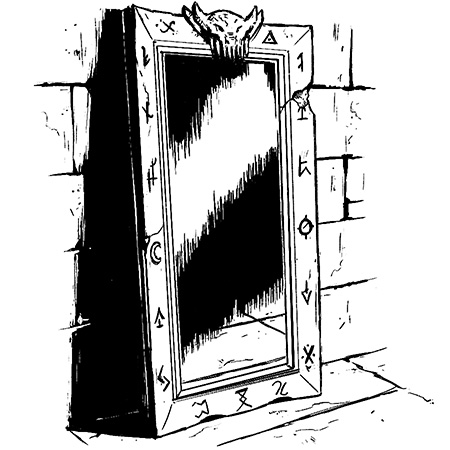
\includegraphics[width=0.7\textwidth,keepaspectratio]{mirror.jpg}\par
\vspace{0.4cm}
{\itshape Who are you?}\par
\vspace*{\fill}
\end{center}

\end{document}